% Hinh quy trinh nghien cuu (flowchart, dap Reviewer D). Ban tieng Anh.
% Bien dich: tectonic fig0_flow_en.tex  ->  fig0_flow_en.pdf
\documentclass[border=2pt]{standalone}
\usepackage{fontspec}
\setmainfont{TeX Gyre Termes}
\usepackage{amsmath}
\usepackage[dvipsnames]{xcolor}
\usepackage{tikz}
\usetikzlibrary{arrows.meta,positioning,calc,fit,backgrounds}
\newcommand{\Lbl}[1]{\textbf{#1}}
\begin{document}
\hyphenpenalty=10000 \exhyphenpenalty=10000
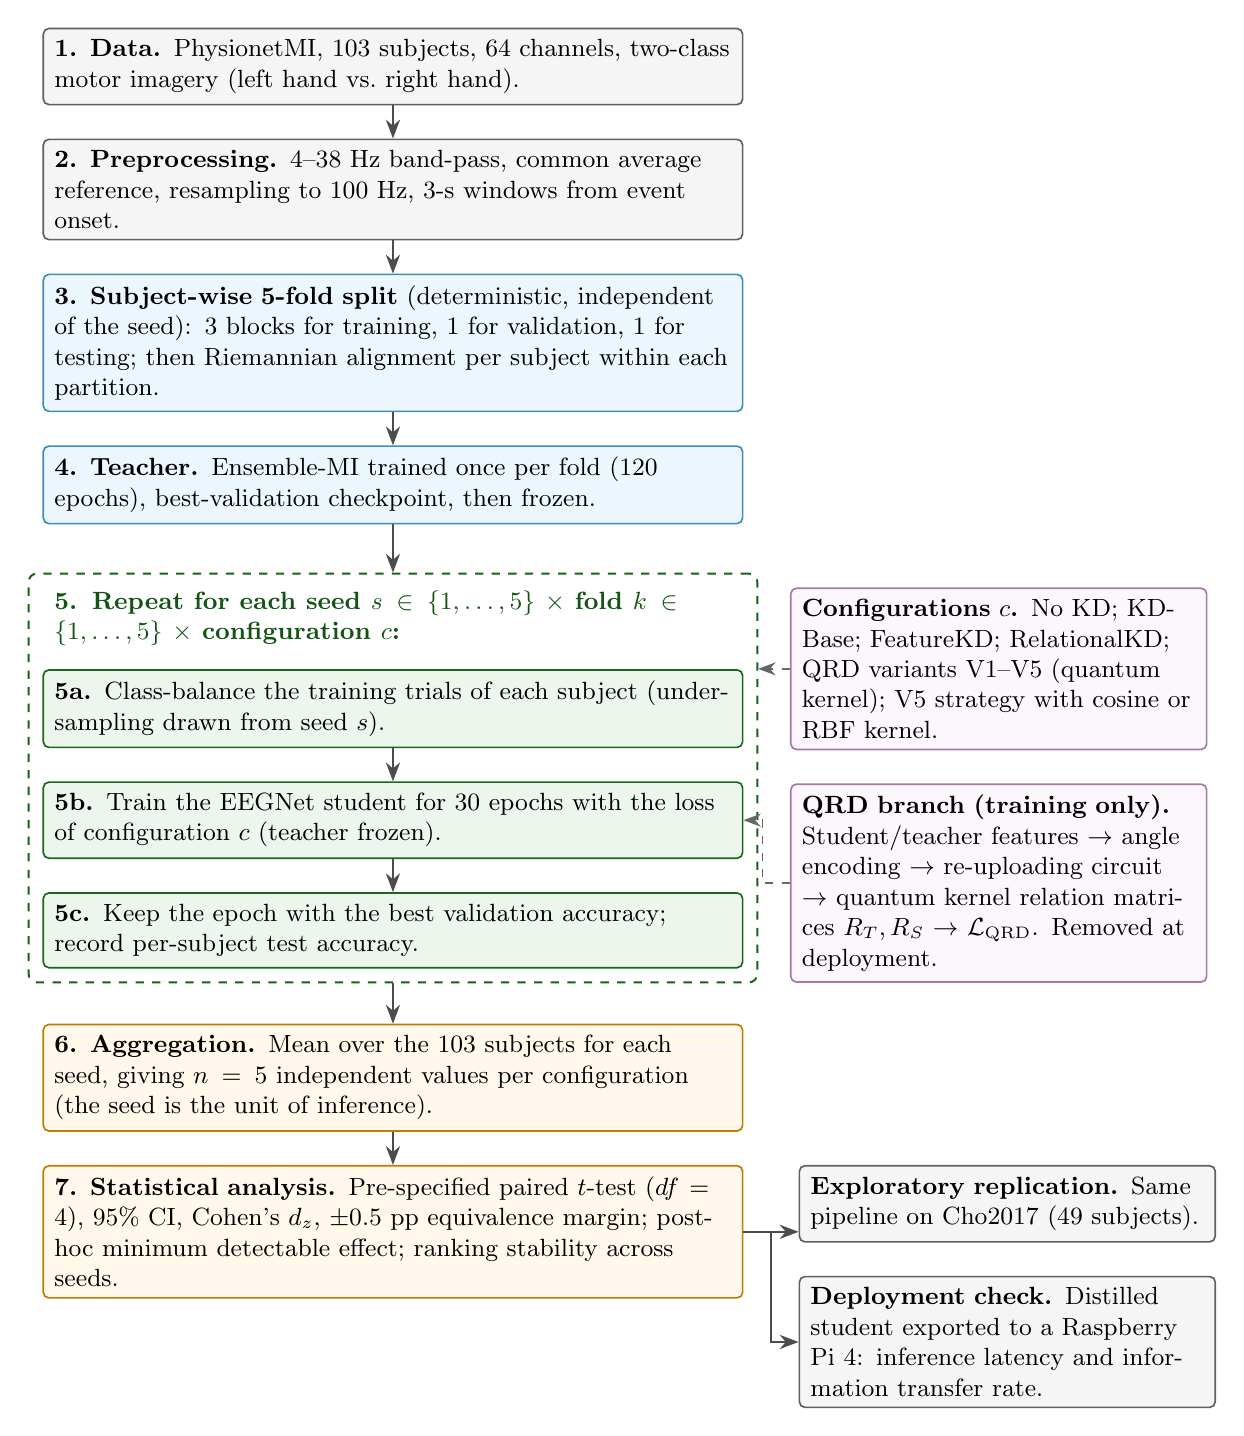
\begin{tikzpicture}[
  font=\small,
  node distance=4.2mm,
  box/.style={draw=#1!75!black, fill=#1!8, rounded corners=2pt, line width=0.6pt,
              text width=8.6cm, align=left, inner sep=4pt},
  side/.style={draw=#1!75!black, fill=#1!8, rounded corners=2pt, line width=0.6pt,
               text width=5.0cm, align=left, inner sep=4pt},
  arr/.style={-{Stealth[length=2.4mm]}, line width=0.7pt, draw=black!70},
  darr/.style={-{Stealth[length=2.2mm]}, line width=0.6pt, draw=black!60, dashed},
]
% ---------------- cot chinh ----------------
\node[box=gray] (data) {\Lbl{1. Data.} PhysionetMI, 103 subjects, 64 channels,
  two-class motor imagery (left hand vs.\ right hand).};
\node[box=gray, below=of data] (prep) {\Lbl{2. Preprocessing.} 4--38 Hz band-pass,
  common average reference, resampling to 100 Hz, 3-s windows from event onset.};
\node[box=Cerulean, below=of prep] (split) {\Lbl{3. Subject-wise 5-fold split}
  (deterministic, independent of the seed): 3 blocks for training, 1 for
  validation, 1 for testing; then Riemannian alignment per subject within
  each partition.};
\node[box=Cerulean, below=of split] (teacher) {\Lbl{4. Teacher.} Ensemble-MI trained
  once per fold (120 epochs), best-validation checkpoint, then frozen.};
% vong lap
\node[text width=8.6cm, align=left, font=\small\bfseries, text=ForestGreen!60!black,
      below=8mm of teacher, inner sep=1pt] (looptitle) {5. Repeat for each seed
      $s\in\{1,\dots,5\}$ $\times$ fold $k\in\{1,\dots,5\}$ $\times$ configuration $c$:};
\node[box=ForestGreen, below=2.5mm of looptitle] (bal) {\Lbl{5a.} Class-balance the
  training trials of each subject (undersampling drawn from seed $s$).};
\node[box=ForestGreen, below=of bal] (train) {\Lbl{5b.} Train the EEGNet student for
  30 epochs with the loss of configuration $c$ (teacher frozen).};
\node[box=ForestGreen, below=of train] (select) {\Lbl{5c.} Keep the epoch with the best
  validation accuracy; record per-subject test accuracy.};
\begin{scope}[on background layer]
  \node[draw=ForestGreen!70!black, dashed, line width=0.7pt, rounded corners=3pt,
        inner sep=5pt, fit=(looptitle)(bal)(train)(select)] (loop) {};
\end{scope}
\node[box=Orange, below=7mm of select] (agg) {\Lbl{6. Aggregation.} Mean over the
  103 subjects for each seed, giving $n=5$ independent values per configuration
  (the seed is the unit of inference).};
\node[box=Orange, below=of agg] (stats) {\Lbl{7. Statistical analysis.} Pre-specified
  paired $t$-test ($df=4$), 95\% CI, Cohen's $d_z$, $\pm 0.5$ pp equivalence
  margin; post-hoc minimum detectable effect; ranking stability across seeds.};

\draw[arr] (data) -- (prep);
\draw[arr] (prep) -- (split);
\draw[arr] (split) -- (teacher);
\draw[arr] (teacher) -- (loop.north -| teacher.south);
\draw[arr] (bal) -- (train);
\draw[arr] (train) -- (select);
\draw[arr] (loop.south -| select.south) -- (agg);
\draw[arr] (agg) -- (stats);

% ---------------- cot phu ----------------
\node[side=Plum, right=7mm of looptitle.north east, anchor=north west] (cfg)
  {\Lbl{Configurations $c$.} No KD; KDBase; FeatureKD; RelationalKD;
  QRD variants V1--V5 (quantum kernel); V5 strategy with cosine or RBF kernel.};
\node[side=Plum, below=of cfg] (qrd) {\Lbl{QRD branch (training only).}
  Student/teacher features $\rightarrow$ angle encoding $\rightarrow$
  re-uploading circuit $\rightarrow$ quantum kernel relation matrices
  $R_T, R_S$ $\rightarrow$ $\mathcal{L}_{\mathrm{QRD}}$. Removed at deployment.};
\node[side=gray, right=7mm of stats.north east, anchor=north west] (cho)
  {\Lbl{Exploratory replication.} Same pipeline on Cho2017 (49 subjects).};
\node[side=gray, below=of cho] (pi) {\Lbl{Deployment check.} Distilled student
  exported to a Raspberry Pi 4: inference latency and information transfer rate.};

\draw[darr] (cfg.west) -- (cfg.west -| loop.east);
\draw[darr] (qrd.west) -- ++(-3.5mm,0) |- (train.east);
\draw[arr] (stats.east) -- (cho.west |- stats.east);
\draw[arr] ($(stats.east)+(3.5mm,0)$) |- (pi.west);
\end{tikzpicture}
\end{document}
